\documentclass[twoside,twocolumn]{article}

\usepackage{blindtext} % Package to generate dummy text throughout this template 
\usepackage{graphicx}
\usepackage[sc]{mathpazo} % Use the Palatino font
\usepackage[T1]{fontenc} % Use 8-bit encoding that has 256 glyphs
\linespread{1.05} % Line spacing - Palatino needs more space between lines
\usepackage{microtype} % Slightly tweak font spacing for aesthetics

\usepackage[english]{babel} % Language hyphenation and typographical rules

\usepackage[hmarginratio=1:1,top=32mm,columnsep=20pt]{geometry} % Document margins
\usepackage[hang, small,labelfont=bf,up,textfont=it,up]{caption} % Custom captions under/above floats in tables or figures
\usepackage{booktabs} % Horizontal rules in tables
\usepackage{graphicx}
\usepackage{lettrine} % The lettrine is the first enlarged letter at the beginning of the text

\usepackage{enumitem} % Customized lists
\setlist[itemize]{noitemsep} % Make itemize lists more compact

\usepackage{abstract} % Allows abstract customization
\renewcommand{\abstractnamefont}{\normalfont\bfseries} % Set the "Abstract" text to bold
\renewcommand{\abstracttextfont}{\normalfont\small\itshape} % Set the abstract itself to small italic text

\usepackage{titlesec} % Allows customization of titles
\renewcommand\thesection{\Roman{section}} % Roman numerals for the sections
\renewcommand\thesubsection{\roman{subsection}} % roman numerals for subsections
\titleformat{\section}[block]{\large\scshape\centering}{\thesection.}{1em}{} % Change the look of the section titles
\titleformat{\subsection}[block]{\large}{\thesubsection.}{1em}{} % Change the look of the section titles

\usepackage{fancyhdr} % Headers and footers
\pagestyle{fancy} % All pages have headers and footers
\fancyhead{} % Blank out the default header
\fancyfoot{} % Blank out the default footer
\fancyhead[C]{Tecnologias de Disponibilidad $\bullet$ Septiembre 2021 $\bullet$ } % Custom header text
\fancyfoot[RO,LE]{\thepage} % Custom footer text

\usepackage{titling} % Customizing the title section

\usepackage{hyperref} % For hyperlinks in the PDF

%----------------------------------------------------------------------------------------
%	TITLE SECTION
%----------------------------------------------------------------------------------------

\setlength{\droptitle}{-4\baselineskip} % Move the title up

\pretitle{\begin{center}\Huge\bfseries} % Article title formatting
\posttitle{\end{center}} % Article title closing formatting
\title{Comparativa de Tecnologias de Disponibilidad en Bases de Datos} % Article title
\author{Carlos Maldonado, Alfredo Huillca, Daniela Soto, Alexander Huallpa, Laura Condori}
\date{\today} % Leave empty to omit a date
\renewcommand{\maketitlehookd}{%

}

%----------------------------------------------------------------------------------------

\begin{document}

% Print the title
\maketitle

%----------------------------------------------------------------------------------------
%	ARTICLE CONTENTS
%----------------------------------------------------------------------------------------

\section{Resumen}

\lettrine[nindent=0em,lines=3] Las bases de 
datos han evolucionado de decenas de megabytes a
 terabytes y aún hasta petabytes. Agregando complejidad
  a la administración y sistematizacion de estas enormes 
  bases de datos. Para ello se utilizan diferentes tecnologías 
  y sistemas que ayudan a facilitar esta tarea. 

La asignación de objetos relacionales es una técnica que le 
permite asignar cada una de las filas de nuestras tablas en la
 base de datos de objetos, donde las columnas de la tabla corresponden 
 a las propiedades de estos objetos. La técnica, utilizada en la
  programación para convertir los tipos de datos con los que trabajan
   en un lenguaje orientado a objetos, los tipos de datos con los que 
   trabajan en un sistema de base de datos relacional para la persistencia
    de datos en el objeto de mapeorelacional. 



%------------------------------------------------

\section{Abstract}


Databases have evolved from tens of megabytes to 
terabytes and even to petabytes. Adding complexity to 
the administration and systematization of these huge databases.
 For this, different technologies and systems are used to help 
 facilitate this task.

Relational object mapping is a technique that allows 
you to map each of the rows of our tables in the object database,
 where the columns of the table correspond to the properties of these
  objects. The technique, used in programming to convert the data types 
  with which they work in an object-oriented language, the data types with
   which they work in a relational database system for the persistence of 
   data in the object of relational mapping .



%------------------------------------------------
\section{Introduccion}



Es bastante difícil proveer una administración apropiada para este
 tipo de bases de datos, tareas de mantenimiento, afinación y respaldo
  se convierten en imposibles; si la base de datos no puede sacarse de
   servicio por un momento, incluso algunas de estas tareas pueden tomar
    varios días al no ser actualizados. 

Debido a esto, la adopción de una tecnología de alta disponibilidad para
 sistemas de base de datos es definitiva para garantizar el exito del sistema.  

Existe una mediana variedad de sistemas de tecnología disponibles en la 
actualidad, dependiendo de su funcionamiento, de su uso o sus requerimientos.
 En este documento daremos un vistazo a fondo a dos de estas tecnologías.  

\section{Desarrollo}

\subsection{Tecnologia Sharding }

Una de las técnicas para el manejo de bases de datos que está 
tomando vida en la comunidad criptográfica actual es el Sharding.
El sharding es una forma de segmentar los 
datos de una base de datos de forma horizontal, es decir, 
partir la base de datos principal en varias en bases de datos 
más pequeñas y repartiendo la información. De esta forma lo que 
se consigue es una partición de datos en diferentes bases que tengan 
cierta homogeneidad, para conseguir una escalabilidad mucho más rápida. 


El sharding se creó con la finalidad de permitir una mayor
 escalabilidad en sistemas distribuidos y descentralizados. 
 Pero en la actualidad, su aplicación en la tecnología blockchain 
 podría mejorar considerablemente los problemas de escalabilidad a 
 los que se enfrentan redes como Bitcoin y Ethereum.

\subsubsection{¿Como Funciona el Sharding?}
Básicamente lo que hace es dividir la red
 en grupos de nodos más pequeños, para que 
 estos se concentren en procesar transacciones 
 de un grupo limitado de usuarios o smart contracts.
  Con ello el sharding logra usar de forma más eficiente
   el poder de los nodos de la red y ofrecer respuestas más
    rápidas a las transacciones.

Estos nodos se encuentran orquestados por un 
protocolo de funcionamiento, que evita que los grupos de 
nodos puedan solaparse en sus funciones. Una medida que agrega seguridad 
a la red y evita conflictos en su funcionamiento.  Finalmente, el aumento en 
la eficiencia tanto en el procesamiento de transacciones, como en la validación
 y almacenamiento de las mismas, repercute en la capacidad global de la red.
  Esto en forma de un aumento significativo en la escalabilidad, velocidad de 
  procesamiento, almacenamiento, 
redundancia y funciones de la red en general.


   
\subsubsection{Sharding y los desafíos a superar}

Sin duda el sharding es una opción poderosa para escalar 
la tecnología blockchain. Pero su aplicación tiene una serie 
de desafíos que deben resolverse.

En primer lugar, usar sharding hace que cada pequeño grupo de
 nodos sea más susceptible de ser atacado. Esto se debe a que
  cada pequeño grupo de nodos mantendría una copia de su sub-cadena
   y al ser más pequeño, un atacante puede dirigir un ataque a estos
    de forma más sencilla para reescribirla o realizar una denegación 
    de servicio. Problemas como el Ataque de 51 por ciento,
 el Ataque de carrera o el Ataque de Vector 76 se hacen más 
 sencillos de llevar a cabo. Después de todo, no atacas a una red
  con miles de nodos, sino algo mucho menor.

Por ejemplo, para realizar un ataque de 51 por ciento
 en una blockchain con sharding solo necesitamos tener bajo 
 control el 5,1 por ciento
  de los nodos totales de la red. Esto se debe,
   a que las redes que usan sharding serían susceptibles 
   al llamado Ataque del 1 por ciento. Lo que significa que solo
    basta con controlar el 1 por ciento
     de un grupo para controlar el poder un grupo de nodos en sharding.
      Esto es un enorme problema de seguridad. Uno que tiene que atenderse
       antes de poder aplicar el sharding en blockchains como Ethereum.

En segundo lugar, nos encontramos con el problema de la selección
 de nodos para la validación. Siendo usuarios de la blockchain podemos
  emitir una transacción y esperamos que esta sea atendida por algún nodo
   dentro del sharding. Sin embargo, la estructura del sharding abre las 
   puertas para que un atacante que controle cierta cantidad de nodos pueda
    validar la transacción en diferentes segmentos de la red al mismo tiempo.
     Como resultado, el atacante podría llevar a cabo ataques de doble gasto.

Sin embargo, esto tiene ya una solución práctica.
 Esta pasa por crear un sistema que permite asignar las 
 transacciones de forma aleatoria a los nodos que forman parte
  de la red. De esta forma, la red velará por asignar transacciones
   a distintos grupos de nodos y que estos procesan la transacción 
   en su momento. El proceso sin embargo introduce una fuerte latencia 
   y otros problemas de seguridad no estudiados a profundidad aún.
\subsubsection{Ventajas del sharding}

En la práctica lo primero que vamos a notar es que el sharding nos ofrece unos 
accesos de gran velocidad. No importa, si por ejemplo disponemos de servidores 
en distintas zonas del mundo, dado que el sharding se ocupa de que se reduzca 
el volumen de latencia y el rendimiento sea superior. Con el sharding vamos a 
poder gestionar mejor las empresas en las que se ha llegado a alcanzar una 
cantidad de datos enorme que ha llevado a que la velocidad de acceso se reduzca 
de forma considerable. Si por el contrario nuestro servidor no tiene tantos datos,
 pero sí registra una gran cantidad de escrituras, también nos veremos 
 beneficiados de ello. Al fin y al cabo, hay que tener en cuenta que las
  escrituras se interpretan como bloqueos en el uso de los recursos, lo que
   acaba derivando en que haya problemas de rendimiento en la forma en la que 
   los usuarios interactúan con nuestro sistema.

El sharding se encuentra presente en la mayor parte de los sistemas actuales,
 desde Hibernate hasta Apache, MongoDB o MySQL a través de distintas 
 implementaciones. Por ejemplo, Oracle NoSQL Database introduce el sharding
  de manera automatizada con expansión online, mientras que la base de datos 
  Spanner de Google lo ofrece por medio de distintas máquinas Paxos.

Otras de las ventajas de este escalado residen en cómo se reduce la cantidad 
de filas en las tablas de las bases de datos, minimizando de manera simultánea
 el tamaño de los índices. El efecto posterior de esto no es solo el aumento de
  espacio liberado, sino también que vamos a comprobar cómo las búsquedas se
   realizan con una mayor rapidez. Además, teniendo en cuenta que el sharding 
   utiliza distintas máquinas para los shards, esto también beneficia a un 
   aumento en el rendimiento.
\subsubsection{Desventajas del Sharding}

Hay expertos que no recomiendan utilizar el sharding en el inicio de un proyecto 
debido a que hay que entender sobre todo cuándo utilizarlo y dentro de qué límites
 de magnitud aprovecharlo. En parte por algunas de las desventajas que podemos 
 comentar, como que la complejidad del SQL se incrementa, llevando a que los 
 desarrolladores tengan que escribir código más elaborado. Este volumen de 
 complejidad no solo se aplica al código, sino que también deriva en que la 
 integridad del sistema se pueda encontrar en mayor riesgo, con distintos 
 factores que pueden sufrir problemas, como el balance y las particiones.

Otra desventaja importante es cómo solo la corrupción que se pueda sufrir 
en uno de los shards del sistema puede llevar a que se produzca un fallo del 
sistema generalizado. Además, los servidores de recuperación están obligados 
a contar con copias de los shards de la base de datos, los backups son más 
complicados de realizar y se introduce una complejidad operacional que lo hace
 todo más complicado en términos globales.
 \subsection{Tecnologia Partitioning}
 Partitioning es una división de base de datos lógica o sus elementos
  constituyentes en partes independientes. La partición de bases de datos
   se hace normalmente por razones de mantenimiento, rendimiento o manejo. 

Una aplicación favorable es en un sistema de administración de bases de datos 
distribuidas. Cada partición puede ser extendida hasta múltiples nodos, y los 
usuarios en el nodo pueden hacer transacciones locales en la partición. Esto 
aumenta el rendimiento en sitios que tienen transacciones regularmente 
involucrando ciertas vistas de datos, y manteniendo la disponibilidad y 
la seguridad. 

El objetivo principal de particionar es ayudar en el mantenimiento de 
tablas grandes y reducir el tiempo de respuesta general para leer y cargar
 datos para operaciones SQL particulares. 
\subsubsection{Particionamiento Vertical en tablas}
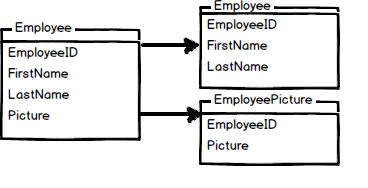
\includegraphics[width=7cm, height=7cm]{Imagenes/img1.png}
El particionamiento vertical de tablas es principalmente usado para 
incrementar el desempeño especialmente en casos cuando una consulta
 retorna todas las columnas de una tabla que contiene un número de
  columnas de texto muy amplio. En este caso, para reducir los tiempos 
  de acceso, las columnas pueden ser divididas a su propia tabla. 
  Otro ejemplo es restringir el acceso a datos sensibles, por ejemplo 
  contraseñas, información salarial, etc.
\subsubsection{Particionamiento Horizontal en tablas.}
El particionamiento horizontal divide una tabla en múltiples tablas que
 contienen el mismo número de columnas, pero menos filas. Por ejemplo, 
 si una tabla contiene un gran número de filas que representan reportes
  mensuales podría ser particionada horizontalmente en tablas por años, 
  con cada tabla representando todos los reportes para un año específico.
   De esta manera las consultas que requieren datos para un año específico
    sólo referenciarán la tabla apropiada. Las tablas deberían ser particionadas
     en una manera que las consultas referencian tan pocas tablas como sea posible.
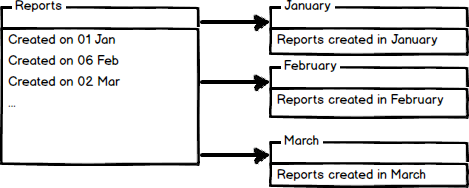
\includegraphics[width=7cm, height=7cm]{Imagenes/img2.png}
\subsubsection{Beneficios del particionamiento}
El particionamiento brinda grandes beneficios al mejorar la capacidad de 
administración, el desempeño y la disponibilidad. No es inusual que el
 particionamiento mejore mucho más el desempeño de ciertas operaciones de
  mantenimiento y consultas. Además, el particionamiento puede reducir 
  enormemente el costo total de propiedad de los datos, al utilizar un
   enfoque de “archivo por niveles” para mantener la información relevante
    más antigua aún online en dispositivos de almacenamiento de bajo costo.
     El particionamiento también permite a los diseñadores y administradores
      de base de datos abordar algunos de los problemas más difíciles planteados
       por las aplicaciones de vanguardia. Es una herramienta clave para crear 
       sistemas de múltiples terabytes o sistemas con requisitos de disponibilidad
        extremadamente altos. 
\subsection{Tecnologia REPLICATION}
Es el proceso de copiar y almacenar datos en múltiples ubicaciones. 
El proceso de replicación puede ser único o continuo, según los requisitos 
de la organización; este último tiene como objetivo garantizar que los datos
 replicados se actualicen periódicamente y sean coherentes con la fuente. 

El propósito principal de la replicación de datos es mejorar la 
disponibilidad y accesibilidad de los datos y la solidez y consistencia 
del sistema. 

El término replicación se refiere a la operación de copiar 
y administrar  objetos de base de datos en múltiples bases de 
datos a  lo largo de un sistema distribuido, en este caso, existen 
varias copias del mismo objeto en diferentes  localidades.  

La replicación es utilizada para mejorar el  rendimiento de 
la base de datos local y brindar alta disponibilidad en el  
sistema; ya que existen  localidades alternas con copias o réplicas 
de los objetos de base de datos.    Por ejemplo, una aplicación puede 
normalmente acceder a la base de  datos  local,  en lugar de un  servidor
 remoto para minimizar el tráfico de red y  lograr un máximo  rendimiento.
  La replicación mejora la disponibilidad de las aplicaciones debido a que 
  provee localidades alternas para el  acceso de los datos. Si una  de las 
  localidades no esta disponible, los usuarios pueden continuar  consultando 
  o modificando la información, en cualquiera de las localidades restantes. En
    otras palabras la replicación provee una excelente alternativa como respuesta
     a fallos a  un tiempo de caída en una localidad particular. 
\begin{itemize}
   \item Rendimiento: El rendimiento es mejorado mediante el uso de cachés en clientes o servidores. El uso de cachés permite mantener copias de los resultados obtenidos en llamadas anteriores, reduciendo el coste de llamadas idénticas. Por otro lado, normalmente, hay más lectura que escritura en una base de datos, por lo que tener varios nodos solo procesando la lectura puede traer un gran beneficio de rendimiento en una base de datos muy consultada.
   \item A prueba de fallos: Con la replicación ganamos tolerancia a diferentes tipos de fallos:
   \begin{itemize}
      \item Fallos en el servidor: Un esclavo estando casi sincrónicamente actualizado puede ser útil en caso de que el nodo maestro caiga, ya que puede reemplazarlo sin detener el servicio. 
      \item Fallos bizantinos: Las fallas bizantinas, son capaces de confundir los sistemas de detección de fallas. 
   \end{itemize}
   \item Fiabilidad: La replicación garantiza que los datos han sido copiados a otro nodo en caso de que el nodo maestro haya sufrido un desperfecto.
   \item Generación de bloqueos: aunque esta es más precisa, también se puede usar para procesos que necesiten leer datos, generando bloqueos. Al hacerlo sobre un esclavo esto no interviene en el funcionamiento de todo el sistema. Es muy usado para, por ejemplo, hacer copias de seguridad o extraer grandes cantidades de datos para generar estadísticas. 
   \item Alta disponibilidad: La proporción de tiempo que el servicio está accesible con tiempos de respuesta razonables es cercana al 100 por ciento. Sin embargo, puede haber fallos en el servidor o desconexiones de red que hagan que la disponibilidad disminuya. 
\end{itemize}
 

La replicación se usa mucho en sistema de acceso a datos por varios motivos: 
\section{Conclusiones}
   \begin{itemize}
      \item Replicación: Para  el logro de alta disponibilidad, requiere un análisis de las tablas empleadas por los  sistemas para poder construir réplicas en la base de datos secundaria. 
      \item Particionamiento: Dividir una gran base de datos monolitica en varias bases de datos mas pequeñas basadas en la cohesión de datos.
      \item Fracmentacion: Dividir una tabla grande de datos horizontalmente, es decir, en filas. Una tabla que contiene cientos de millones de filas se puede dividir en varias tablas que contienen 1 millón de filas cada una. 
   \end{itemize}
\section{Recomendaciones}
Para  implementar alta disponibilidad en un  sistema, es necesario  comprender el nivel de disponibilidad que los usuarios  requieren en las  aplicaciones y  su impacto financiero, por lo que se debe  definir un acuerdo de nivel de servicio donde se debe realizar  una revisión de   las aplicaciones críticas y los horarios de operación, así como el costo de una eventual falla del sistema, tanto desde la perspectiva del negocio como  a nivel de tecnología.  

 

La revisión de los recursos tecnológicos actuales de una compañía es obligatoria para   un director de tecnología, ante  el desafío de elevar los niveles de disponibilidad de los sistemas.  

 

Para la implementación de un sistema de base de datos de alta disponibilidad  de bajo presupuesto,   la replicación y la base de datos en espera, constituyen una excelente alternativa. 
%----------------------------------------------------------------------------------------
%	REFERENCE LIST
%----------------------------------------------------------------------------------------

\begin{thebibliography}{XXX0000}
	\bibitem - Raquel García (2020) Sharding, ventajas y desventajas de su aplicación, Recuperado 19 de Setiembre del 2021, de: https://blog.mdcloud.es/sharding-ventajas-y-desventajas/ 
	\bibitem - Ankush Thakur (2020) ¿Qué es MongoDB Sharding y las mejores prácticas?, Recuperado 19 de Setiembre del 2021, de: https://geekflare.com/es/mongodb-sharding-best-practices/
	\bibitem - José Maldonado (2020) Sharding, una oportunidad para la escalabilidad distribuida, Recuperado 19 de Setiembre del 2021, de: https://es.cointelegraph.com/explained/sharding-an-opportunity-for-distributed-scalability 
	\bibitem - Asad Ali (2020) Sharding en MongoDB: una guía práctica, Recuperado 19 de Setiembre del 2021, de: https://geekflare.com/es/mongodb-sharding/
	\bibitem - Rubén Colomer, (27 febrero 2021) ¿Qué es sharding? ¿Qué ventajas e inconvenientes tiene?, Recuperado 19 de Setiembre del 2021, de: https://www.lemmingatwork.com/inversiones/criptomonedas/que-es-sharding/  
	\bibitem - Craig S. Mullins (2018) ¿Cuáles son los métodos de escalabilidad de la base de datos?, Recuperado 19 de Setiembre del 2021, de: https://nuodb.com/blog/what-are-database-scalability-methods 
	\bibitem - Oracle (Junio de 2007) Particionamiento en Oracle Database 11g, Recuperado 19 de Setiembre del 2021, de: https://www.oracle.com/technetwork/es/documentation/317489-esa.pdf  
	\bibitem - Milica Medic (December 4, 2015) Particionamiento de tablas de bases de datos en SQL Server, Recuperado 19 de Setiembre del 2021, de: https://www.sqlshack.com/es/particionamiento-de-tablas-de-bases-de-datos-en-sql-server/ 
	\end{thebibliography}

%----------------------------------------------------------------------------------------

\end{document}